% =============================================================
% Lecture: Panel Data Econometrics
% Topic: Lecture 2 - Difference-in-Differences and Synthetic Control
% Course: Quantitative Economics, Vilnius University
% Author: Swapnil Singh
% =============================================================
\documentclass[10pt]{beamer}

\usepackage[T1]{fontenc}
\usepackage{graphicx}
\usepackage{booktabs}
\usepackage{tabularx}
\usepackage{array}
\usepackage{ragged2e}
\usepackage{appendixnumberbeamer}
\usepackage{amsmath,amssymb,amsfonts}
\usepackage{mathtools}
\usepackage{hyperref}
\usepackage{tikz}
\usetikzlibrary{arrows.meta,positioning,calc}

\usetheme{SimplePlus}

\title{Panel Data Econometrics}
\subtitle{Lecture 2: Difference-in-Differences and Synthetic Control}
\author{Swapnil Singh}
\institute{Lietuvos Bankas \and Kaunas University of Technology}
\date{Vilnius University, 2026}

\DeclareMathOperator{\Cov}{Cov}
\DeclareMathOperator{\Var}{Var}
\newcommand{\E}{\mathbb{E}}
\newcommand{\ATT}{\operatorname{ATT}}

\begin{document}

\begin{frame}[plain]
  \titlepage
  \vfill
  {\scriptsize\color{gray} Based on \texttt{lectures/panel-data-notes.tex}.}
\end{frame}

\begin{frame}{Roadmap}
\tableofcontents
\end{frame}

\section{Difference-in-Differences}

\begin{frame}{The comparison problem in policy evaluation}
\label{slide:did_compare}
\small
\begin{block}{Typical empirical question}
Did a reform, subsidy, tax change, or regulation alter employment, wages, prices, schooling, health, or firm behavior?
\end{block}

\begin{columns}[T]
\begin{column}{0.49\textwidth}
\begin{alertblock}{The object we observe}
For treated units after the policy, we observe the realized outcome:
\[
Y_{i,post}(1).
\]
\end{alertblock}
\end{column}
\begin{column}{0.49\textwidth}
\begin{alertblock}{The object we need but never observe}
For those same treated units, we do not observe the untreated outcome:
\[
Y_{i,post}(0).
\]
\end{alertblock}
\end{column}
\end{columns}

\begin{exampleblock}{Why panel data help}
If we observe treated and untreated units before and after treatment, we can use untreated changes as evidence about the missing counterfactual path. Difference-in-differences is exactly this comparison strategy written carefully.
\end{exampleblock}
\end{frame}

\begin{frame}{Potential outcomes: what is observed and what is missing?}
\label{slide:did_po_setup}
\small
For each unit and period, let
\[
Y_{it}(0)=\text{outcome without treatment},
\qquad
Y_{it}(1)=\text{outcome with treatment}.
\]

\begin{columns}[T]
\begin{column}{0.49\textwidth}
\begin{block}{Pre period}
Before treatment starts, both groups are untreated, so
\[
Y_{i,pre}=Y_{i,pre}(0).
\]
\end{block}
\end{column}
\begin{column}{0.49\textwidth}
\begin{block}{Post period}
After treatment begins,
\[
Y_{i,post}=
\begin{cases}
Y_{i,post}(1), & D_i=1,\\[0.3em]
Y_{i,post}(0), & D_i=0.
\end{cases}
\]
\end{block}
\end{column}
\end{columns}

\begin{alertblock}{The missing-data problem}
For treated units we observe $Y_{i,post}(1)$ but not $Y_{i,post}(0)$. The entire DiD design is an attempt to recover
\[
\E[Y_{i,post}(0)\mid D_i=1].
\]
\end{alertblock}
\end{frame}

\begin{frame}{Why selection bias appears immediately}
\label{slide:did_selection}
\small
\begin{block}{What goes wrong with a simple treated-control comparison?}
Even before treatment starts, treated and untreated units may differ because treatment is rarely assigned at random.
\end{block}

\begin{columns}[T]
\begin{column}{0.48\textwidth}
\begin{exampleblock}{Selection on levels}
Units selected into treatment may have systematically different baseline outcomes:
\[
\E[Y_{pre}(0)\mid D=1]\neq \E[Y_{pre}(0)\mid D=0].
\]
\end{exampleblock}
\end{column}
\begin{column}{0.48\textwidth}
\begin{exampleblock}{Selection on trends}
More seriously, the treated group may have followed a different untreated path even without treatment:
\begin{align*} 
\E[Y_{post}(0)-Y_{pre}(0)\mid D=1]\neq \\ \E[Y_{post}(0)-Y_{pre}(0)\mid D=0].
\end{align*}
\end{exampleblock}
\end{column}
\end{columns}

\begin{alertblock}{Why this matters for DiD}
Selection on levels is not fatal for DiD because differencing can remove permanent gaps. Selection on untreated trends is fatal because it breaks the counterfactual trend comparison.
\end{alertblock}
\end{frame}

\begin{frame}{Why the target parameter is the ATT}
\label{slide:did_att_target}
\small
\begin{block}{Natural estimand in policy evaluation}
When treatment is applied to a particular group, the most natural causal parameter is the effect on those actually treated:
\[
\ATT
=
\E\!\left[Y_{i,post}(1)-Y_{i,post}(0)\mid D_i=1\right].
\]
\end{block}

\begin{columns}[T]
\begin{column}{0.48\textwidth}
\textbf{Why ATT rather than ATE?}

The policy is applied to a specific group, not randomly assigned to the whole population. The empirical problem is therefore about the treated group's missing untreated outcome.
\end{column}
\begin{column}{0.48\textwidth}
\textbf{Observed and missing pieces}

For treated units after treatment,
\[
\E[Y_{post}(1)\mid D=1]
\]
is observed, while
\[
\E[Y_{post}(0)\mid D=1]
\]
is not.
\end{column}
\end{columns}

\medskip
\begin{alertblock}{Transition}
Rewrite an observed contrast so it equals the ATT plus a bias term.
\end{alertblock}
\end{frame}

\begin{frame}{From the observed DiD contrast to the ATT}
\label{slide:did_att_bridge}
\small
Start from the population DiD contrast:
\[
\Delta^{DiD}
=
\Big(\E[Y_{post}\mid D=1]-\E[Y_{pre}\mid D=1]\Big)
-\Big(\E[Y_{post}\mid D=0]-\E[Y_{pre}\mid D=0]\Big).
\]

\begin{block}{Substitute the potential outcomes mapping}
Because the treated group is untreated in the pre period and treated in the post period,
\[
\E[Y_{post}\mid D=1]-\E[Y_{pre}\mid D=1]
=
\E[Y_{post}(1)-Y_{pre}(0)\mid D=1].
\]
For the control group,
\[
\E[Y_{post}\mid D=0]-\E[Y_{pre}\mid D=0]
=
\E[Y_{post}(0)-Y_{pre}(0)\mid D=0].
\]
\end{block}

\begin{exampleblock}{Decomposition}
After adding and subtracting $\E[Y_{post}(0)\mid D=1]$, the DiD contrast becomes
\[
\Delta^{DiD}
=
\ATT
+\Big(
\E[Y_{post}(0)-Y_{pre}(0)\mid D=1]
-\E[Y_{post}(0)-Y_{pre}(0)\mid D=0]
\Big).
\]
\end{exampleblock}

\hfill\hyperlink{app:did-att}{\beamerbutton{ATT Derivation}}
\end{frame}

\begin{frame}{Why the two naive comparisons fail}
\label{slide:did_naive}
\small
\begin{columns}[T]
\begin{column}{0.48\textwidth}
\begin{block}{Before-after for treated units}
\[
\E[Y_{post}\mid D=1]-\E[Y_{pre}\mid D=1]
\]
This is not yet causal because it mixes the treatment effect with:
\begin{itemize}
  \item macro shocks,
  \item secular trends,
  \item seasonality or business-cycle movements,
  \item any other change that would have happened anyway.
\end{itemize}
\end{block}
\end{column}
\begin{column}{0.48\textwidth}
\begin{block}{Treated-control comparison after treatment}
\[
\E[Y_{post}\mid D=1]-\E[Y_{post}\mid D=0]
\]
This also fails because it mixes the treatment effect with:
\begin{itemize}
  \item permanent group differences,
  \item selection into treatment,
  \item distinct baseline levels,
  \item structural heterogeneity across units.
\end{itemize}
\end{block}
\end{column}
\end{columns}

\begin{alertblock}{Wooldridge-style lesson}
Neither comparison isolates the policy effect on its own. DiD works by differencing away both common time shocks and permanent group differences, provided the control group is a credible trend benchmark.
\end{alertblock}
\end{frame}

\begin{frame}{The canonical 2x2 design}
\label{slide:did_2x2}
\small
\[
\hat{\delta}^{DiD}
=
(\bar{Y}_{1,post}-\bar{Y}_{1,pre})-(\bar{Y}_{0,post}-\bar{Y}_{0,pre}).
\]

\begin{table}
\centering
\begin{tabular}{lcc}
\toprule
& Pre & Post \\
\midrule
Control & $\bar{Y}_{0,pre}$ & $\bar{Y}_{0,post}$ \\
Treated & $\bar{Y}_{1,pre}$ & $\bar{Y}_{1,post}$ \\
\bottomrule
\end{tabular}
\end{table}

\begin{block}{Read the estimator in words}
\begin{enumerate}
  \item Compute how much the treated group changes.
  \item Compute how much the control group changes.
  \item Attribute the \emph{excess} change of the treated group to treatment.
\end{enumerate}
\end{block}

\begin{exampleblock}{Economic intuition}
The control group is not used because it looks identical to the treated group. It is used because its \emph{change over time} is taken to proxy for the untreated change the treated group would have experienced.
\end{exampleblock}

\hfill\hyperlink{app:did-reg}{\beamerbutton{Algebra}}
\end{frame}

\begin{frame}{Visual intuition: a trend comparison, not a level comparison}
\label{slide:did_plot}
\centering
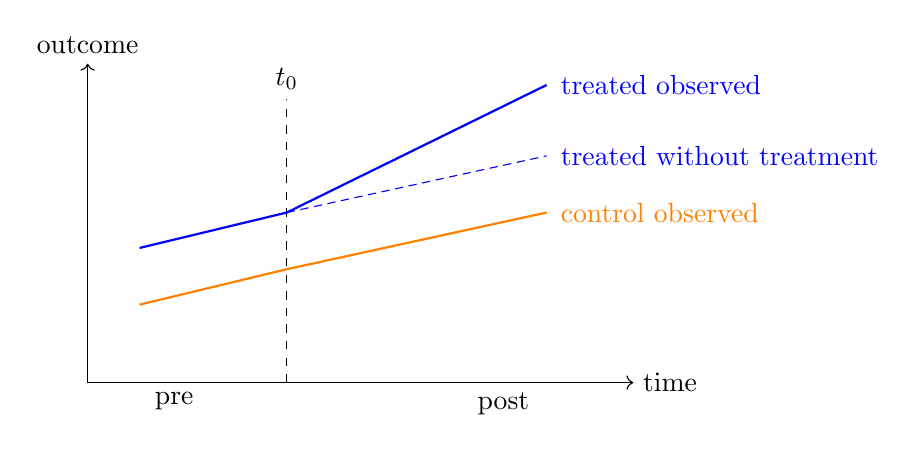
\begin{tikzpicture}[x=1.1cm,y=0.9cm]
\draw[->] (0,0) -- (6.3,0) node[right] {time};
\draw[->] (0,0) -- (0,4.5) node[above] {outcome};
\draw[dashed] (2.3,0) -- (2.3,4.0);
\node[below] at (1.0,0) {pre};
\node[below] at (4.8,0) {post};
\node[above] at (2.3,4.0) {$t_0$};

\draw[thick,blue] (0.6,1.9) -- (2.3,2.4) -- (5.3,4.2);
\draw[thick,orange] (0.6,1.1) -- (2.3,1.6) -- (5.3,2.4);
\draw[densely dashed,blue] (2.3,2.4) -- (5.3,3.2);

\node[blue,right] at (5.35,4.2) {treated observed};
\node[orange,right] at (5.35,2.4) {control observed};
\node[blue,right] at (5.35,3.2) {treated without treatment};
\end{tikzpicture}

\vspace{0.5em}
\begin{block}{What DiD is filling in}
The dashed blue segment is the missing untreated path for the treated group. DiD says: use the control group's observed change to approximate that missing counterfactual change.
\end{block}
\end{frame}

\begin{frame}{Parallel trends is exactly the condition that kills the bias term}
\label{slide:did_pt}
\small
\[
\E[Y_{post}(0)-Y_{pre}(0)\mid D=1]
=
\E[Y_{post}(0)-Y_{pre}(0)\mid D=0].
\]

\begin{block}{Interpretation}
Absent treatment, the treated and control groups would have experienced the same average change in untreated potential outcomes.
\end{block}

\begin{columns}[T]
\begin{column}{0.49\textwidth}
\begin{exampleblock}{What the assumption allows}
\begin{itemize}
  \item different baseline levels;
  \item permanent treated-control gaps;
  \item selection on levels.
\end{itemize}
\end{exampleblock}
\end{column}
\begin{column}{0.49\textwidth}
\begin{alertblock}{What the assumption rules out}
\begin{itemize}
  \item different untreated trends;
  \item treated-specific shocks at treatment time;
  \item anticipation in the pre period.
\end{itemize}
\end{alertblock}
\end{column}
\end{columns}

\begin{exampleblock}{Bottom line}
Under parallel trends, the bias term on the previous slide is zero, so the DiD contrast identifies the ATT.
\end{exampleblock}
\end{frame}

\begin{frame}{What parallel trends does and does not mean}
\label{slide:did_pt_interpret}
\small
\begin{columns}[T]
\begin{column}{0.48\textwidth}
\begin{block}{It does \emph{not} mean}
\begin{itemize}
  \item equal levels in the pre period;
  \item identical covariates in treated and control groups;
  \item identical observed post-treatment outcomes;
  \item no heterogeneity in treatment effects.
\end{itemize}
\end{block}
\end{column}
\begin{column}{0.48\textwidth}
\begin{block}{It \emph{does} mean}
\begin{itemize}
  \item the untreated paths move in parallel on average;
  \item the control group's change is informative about the treated group's missing untreated change;
  \item the design lives or dies on a trend comparison.
\end{itemize}
\end{block}
\end{column}
\end{columns}

\begin{alertblock}{Most common student error}
Students often look only at levels and say ``the groups are too different.'' That is not the right objection. The relevant question is whether untreated \emph{trends} are credibly comparable.
\end{alertblock}
\end{frame}

\begin{frame}{When is parallel trends more plausible?}
\label{slide:did_design}
\small
\begin{columns}[T]
\begin{column}{0.49\textwidth}
\begin{block}{Features that help}
\begin{itemize}
  \item similar institutional environment;
  \item common exposure to macro shocks;
  \item long pre-treatment history;
  \item treatment timing driven by policy rules rather than group-specific shocks;
  \item outcome trends that already move similarly before treatment.
\end{itemize}
\end{block}
\end{column}
\begin{column}{0.49\textwidth}
\begin{alertblock}{Features that damage credibility}
\begin{itemize}
  \item treated units already drifting away before treatment;
  \item anticipation before formal implementation;
  \item spillovers from treated to control units;
  \item policy bundles introduced at the same time;
  \item compositional changes caused by the policy itself.
\end{itemize}
\end{alertblock}
\end{column}
\end{columns}

\begin{exampleblock}{Design principle}
Difference-in-differences is not identified by the regression package. It is identified by a credible argument that the control group's trend stands in for the treated group's missing untreated trend.
\end{exampleblock}
\end{frame}

\begin{frame}{Regression representation and the link to fixed effects}
\label{slide:did_reg}
\small
The canonical two-period DiD regression is
\[
Y_{it} = \alpha + \gamma D_i + \lambda Post_t + \delta(D_i\times Post_t) + u_{it}.
\]

\begin{columns}[T]
\begin{column}{0.49\textwidth}
\begin{block}{Coefficient meanings}
\begin{itemize}
  \item $\alpha$: control mean in the pre period;
  \item $\gamma$: permanent treated-control gap;
  \item $\lambda$: common post shock;
  \item $\delta$: DiD contrast.
\end{itemize}
\end{block}
\end{column}
\begin{column}{0.49\textwidth}
\begin{block}{Panel-data view}
This is a special case of two-way fixed effects:
\[
Y_{it}=\alpha_i+\lambda_t+\delta W_{it}+u_{it},
\]
where $W_{it}=1$ only for treated units after treatment.
\end{block}
\end{column}
\end{columns}

\begin{exampleblock}{Interpretation}
The regression is bookkeeping. The causal content still comes from the potential-outcomes argument and the parallel-trends assumption, not from the mere presence of an interaction term.
\end{exampleblock}

\hfill\hyperlink{app:did-reg}{\beamerbutton{Coefficient Algebra}}
\end{frame}

\begin{frame}{Event studies: diagnosis and substance}
\label{slide:eventstudy}
\small
For staggered or dynamic settings, a common specification is
\[
Y_{it} = \alpha_i + \lambda_t + \sum_{k\neq -1}\beta_k 1\{t-G_i=k\}+u_{it},
\]
where $G_i$ is the treatment date and $k=-1$ is the omitted reference period.

\begin{columns}[T]
\begin{column}{0.49\textwidth}
\begin{block}{Why we look at leads}
Coefficients for periods before treatment are a diagnostic for pre-treatment divergence. Large lead effects undermine the maintained trend comparison.
\end{block}
\end{column}
\begin{column}{0.49\textwidth}
\begin{block}{Why we look at lags}
Coefficients after treatment show whether effects build gradually, fade out, or remain persistent. That is economic content, not just a robustness check.
\end{block}
\end{column}
\end{columns}

\begin{alertblock}{Important restraint}
Failing to reject zero pre-treatment leads is not proof of identification. Small samples, noisy outcomes, and weak pre-period information can make a bad design look quiet.
\end{alertblock}
\end{frame}

\begin{frame}{Modern caution: staggered adoption and two-way fixed effects}
\label{slide:did_twfe}
\small
\begin{block}{What goes wrong in staggered designs}
With staggered adoption, a standard TWFE regression can compare newly treated units to already treated units. That contaminates the control group when effects vary across cohorts or over event time.
\end{block}

\begin{columns}[T]
\begin{column}{0.49\textwidth}
\begin{exampleblock}{Symptoms}
\begin{itemize}
  \item hard-to-interpret weighted averages;
  \item negative or odd comparison weights;
  \item already-treated units acting as controls.
\end{itemize}
\end{exampleblock}
\end{column}
\begin{column}{0.49\textwidth}
\begin{exampleblock}{Better instinct}
Ask in each period: who is compared to whom? If already-treated units help form the control group, the coefficient is no longer a simple average treatment effect.
\end{exampleblock}
\end{column}
\end{columns}

\begin{alertblock}{Practical takeaway}
In staggered settings, cohort-time or group-time ATT estimators are often preferable to a single TWFE coefficient.
\end{alertblock}
\end{frame}

\begin{frame}{A concrete application blueprint}
\label{slide:did_app}
\small
\begin{block}{Example: labor-market reform across regions}
\begin{itemize}
  \item Units: regions or states.
  \item Outcome: employment rate or log employment.
  \item Treatment: reform adopted after year $t_0$.
  \item Control group: untreated regions over the same horizon.
\end{itemize}
\end{block}

\begin{columns}[T]
\begin{column}{0.49\textwidth}
\begin{exampleblock}{Questions the paper must answer}
\begin{enumerate}
  \item Why are untreated regions a good trend benchmark?
  \item Is reform timing related to local shocks?
  \item Do pre-treatment trends look similar?
  \item Are spillovers likely?
\end{enumerate}
\end{exampleblock}
\end{column}
\begin{column}{0.49\textwidth}
\begin{exampleblock}{Inference questions}
\begin{enumerate}
  \item At what level does treatment vary?
  \item At what level might shocks be correlated?
  \item Should standard errors be clustered by state, region, or both?
  \item How many treated clusters are there?
\end{enumerate}
\end{exampleblock}
\end{column}
\end{columns}
\end{frame}

\section{Synthetic Control}

\begin{frame}{Why synthetic control enters the conversation}
\label{slide:sc_motivation}
\small
\begin{block}{The DiD control-group problem}
Sometimes there is only one treated unit, or very few treated units, and no untreated unit is a convincing comparison by itself.
\end{block}

\begin{exampleblock}{Canonical use case}
Suppose one state adopts a major tobacco-control law. Which untreated state is the right counterfactual? California is not well matched by Nevada; Nevada is not well matched by Oregon; and choosing one comparison state by eye is not persuasive.
\end{exampleblock}

\begin{alertblock}{Synthetic-control idea}
Instead of selecting one donor unit, construct a weighted average of untreated donor units that reproduces the treated unit's pre-treatment path as closely as possible.
\end{alertblock}
\end{frame}

\begin{frame}{Core idea of synthetic control}
\label{slide:sc_idea}
\small
Let unit $1$ be treated and units $j=2,\ldots,J+1$ be untreated donors. The synthetic untreated path is
\[
\widehat{Y}_{1t}(0)
=
\sum_{j=2}^{J+1} w_j Y_{jt},
\qquad
w_j\ge 0,
\qquad
\sum_{j=2}^{J+1} w_j = 1.
\]

\begin{columns}[T]
\begin{column}{0.49\textwidth}
\begin{block}{Why the weights are restricted}
Nonnegative weights that sum to one keep the synthetic unit inside the support of the donor pool and prevent wild extrapolation.
\end{block}
\end{column}
\begin{column}{0.49\textwidth}
\begin{block}{How to read the construction}
Synthetic control is not ``the best regression fit'' in the usual sense. It is a transparent, weighted counterfactual built to match the treated unit before treatment.
\end{block}
\end{column}
\end{columns}
\end{frame}

\begin{frame}{Potential outcomes and the synthetic-control estimand}
\label{slide:sc_po}
\small
If treatment starts after $T_0$, then for post-treatment dates $t>T_0$ the effect for the treated unit is
\[
\tau_{1t}=Y_{1t}(1)-Y_{1t}(0).
\]

\begin{block}{Estimator}
Because $Y_{1t}(0)$ is unobserved, synthetic control replaces it with the weighted donor combination:
\[
\hat{\tau}_{1t}
=
Y_{1t}-\sum_{j=2}^{J+1}\hat{w}_j Y_{jt},
\qquad t>T_0.
\]
\end{block}

\begin{alertblock}{Parallel with DiD}
DiD uses the \emph{average change} of the control group to proxy for the missing untreated path. Synthetic control uses a \emph{weighted untreated unit} to proxy for the missing untreated path. The target remains the same sort of object: an unobserved untreated outcome.
\end{alertblock}
\end{frame}

\begin{frame}{How the weights are chosen and why pre-treatment fit matters}
\label{slide:sc_objective}
\small
Let $X_1$ collect pre-treatment characteristics and lagged outcomes for the treated unit, and let $X_0$ be the corresponding donor matrix. Choose weights by solving
\[
\min_W (X_1-X_0W)'V(X_1-X_0W)
\]
subject to
\[
w_j\ge 0,
\qquad
\sum_{j=2}^{J+1} w_j = 1.
\]

\begin{columns}[T]
\begin{column}{0.49\textwidth}
\begin{block}{Why lagged outcomes matter}
Pre-treatment outcomes absorb a great deal of information about observed and unobserved determinants of the untreated path.
\end{block}
\end{column}
\begin{column}{0.49\textwidth}
\begin{alertblock}{Why fit is central}
If the synthetic unit cannot reproduce the treated unit before treatment, there is little reason to trust it after treatment.
\end{alertblock}
\end{column}
\end{columns}

\hfill\hyperlink{app:sc-geom}{\beamerbutton{Convex-Hull Intuition}}
\end{frame}

\begin{frame}{What a convincing synthetic-control graph looks like}
\label{slide:sc_plot}
\centering
\begin{tikzpicture}[x=0.95cm,y=0.8cm]
\draw[->] (0,0) -- (8.5,0) node[right] {time};
\draw[->] (0,0) -- (0,4.6) node[above] {outcome};
\draw[dashed] (5.2,0) -- (5.2,4.1);
\node[below] at (2.2,0) {pre};
\node[below] at (7.0,0) {post};
\node[above] at (5.2,4.1) {$T_0$};

\draw[thick,blue] (0.6,1.2) -- (1.5,1.5) -- (2.4,1.9) -- (3.3,2.1) -- (4.2,2.5) -- (6.1,3.0) -- (7.1,3.5);
\draw[thick,orange] (0.6,1.1) -- (1.5,1.5) -- (2.4,1.9) -- (3.3,2.1) -- (4.2,2.5) -- (6.1,2.6) -- (7.1,2.5);

\node[blue,right] at (7.2,3.5) {treated};
\node[orange,right] at (7.2,2.5) {synthetic};
\end{tikzpicture}

\vspace{0.5em}
\begin{block}{Desired pattern}
Very close tracking before treatment, then a sustained post-treatment divergence. The closer the pre-treatment fit, the stronger the visual case that the synthetic path is approximating the missing untreated outcome.
\end{block}
\end{frame}

\begin{frame}{Diagnostics, placebos, and design discipline}
\label{slide:sc_placebo}
\small
\begin{columns}[T]
\begin{column}{0.49\textwidth}
\begin{block}{Core diagnostics}
\begin{itemize}
  \item treated path versus synthetic path;
  \item post-treatment gap plot;
  \item pre-treatment balance and fit statistics;
  \item leave-one-out donor checks.
\end{itemize}
\end{block}
\end{column}
\begin{column}{0.49\textwidth}
\begin{block}{Placebo logic}
Pretend each donor unit was treated, build its synthetic control, and compare the treated-unit gap with these placebo gaps. The treated-unit effect should stand out relative to placebos with similar pre-treatment fit.
\end{block}
\end{column}
\end{columns}

\begin{alertblock}{Same principle as in DiD}
This remains a counterfactual-design argument. Optimization delivers weights, but it does not by itself deliver credibility. Credibility still comes from the donor pool, the fit, and the institutional story.
\end{alertblock}
\end{frame}

\begin{frame}{Synthetic control versus DiD}
\label{slide:sc_vs_did}
\small
\begin{table}
\centering
\begin{tabular}{p{0.22\textwidth}p{0.29\textwidth}p{0.29\textwidth}}
\toprule
& Difference-in-differences & Synthetic control \\
\midrule
Comparison object & untreated group trend & weighted donor combination \\
Main identifying emphasis & parallel trends in untreated outcomes & ability to reconstruct the treated unit before treatment \\
Most natural setting & many treated and control units & one or a few treated units with long pre-treatment history \\
Main failure mode & bad trend comparison & poor donor support or poor fit \\
\bottomrule
\end{tabular}
\end{table}

\begin{exampleblock}{Unifying theme}
Both methods are trying to recover the missing untreated outcome. They differ in how they construct the comparison object.
\end{exampleblock}
\end{frame}

\begin{frame}{Lecture summary}
\label{slide:summary}
\small
\begin{enumerate}
  \item Difference-in-differences is a trend-comparison design for recovering the treated group's missing untreated post-treatment outcome.
  \item In the potential-outcomes framework, the natural estimand is the ATT.
  \item The population DiD contrast equals the ATT plus a difference in untreated trends; parallel trends is exactly the assumption that sets that bias term to zero.
  \item Event studies and staggered-adoption settings require careful thought about who is compared to whom.
  \item Synthetic control addresses the same counterfactual problem when no single untreated unit is a persuasive control.
\end{enumerate}

\begin{alertblock}{Unifying principle}
Good causal panel work is not a search for a fashionable specification. It is a search for a convincing answer to one question: what is the best available approximation to the untreated outcome we cannot observe?
\end{alertblock}
\end{frame}

\appendix

\section*{Appendix}

\begin{frame}{Appendix: Why the interaction coefficient is the DiD contrast}
\label{app:did-reg}
\small
From
\[
Y_{it} = \alpha + \gamma D_i + \lambda Post_t + \delta(D_i\times Post_t)+u_{it},
\]
the four cell means are
\[
\mu_{00}=\alpha,\quad
\mu_{10}=\alpha+\gamma,\quad
\mu_{01}=\alpha+\lambda,\quad
\mu_{11}=\alpha+\gamma+\lambda+\delta.
\]
Therefore
\begin{align*}
(\mu_{11}-\mu_{10})-(\mu_{01}-\mu_{00})
&=
(\alpha+\gamma+\lambda+\delta-\alpha-\gamma) \\
&\quad -(\alpha+\lambda-\alpha) \\
&= \delta.
\end{align*}
So the interaction coefficient is exactly the population DiD contrast.
\hfill\hyperlink{slide:did_reg}{\beamerbutton{Back}}
\end{frame}

\begin{frame}{Appendix: Deriving the ATT under parallel trends}
\label{app:did-att}
\small
Start from
\[
\Delta^{DiD}
=
\Big(\E[Y_{post}\mid D=1]-\E[Y_{pre}\mid D=1]\Big)
-\Big(\E[Y_{post}\mid D=0]-\E[Y_{pre}\mid D=0]\Big).
\]
Substitute observed outcomes using the potential-outcomes mapping:
\begin{align*}
\Delta^{DiD}
&=
\Big(\E[Y_{post}(1)\mid D=1]-\E[Y_{pre}(0)\mid D=1]\Big) \\
&\quad -\Big(\E[Y_{post}(0)\mid D=0]-\E[Y_{pre}(0)\mid D=0]\Big).
\end{align*}
Now add and subtract $\E[Y_{post}(0)\mid D=1]$:
\[
\Delta^{DiD}
=
\ATT
+
\Big(
\E[Y_{post}(0)-Y_{pre}(0)\mid D=1]
-\E[Y_{post}(0)-Y_{pre}(0)\mid D=0]
\Big).
\]
Under parallel trends, the bracketed term is zero, so
\[
\Delta^{DiD}=\ATT.
\]
\hfill\hyperlink{slide:did_att_bridge}{\beamerbutton{Back}}
\end{frame}

\begin{frame}{Appendix: Convex-hull intuition in synthetic control}
\label{app:sc-geom}
\small
The restrictions
\[
w_j\ge 0,
\qquad
\sum_{j=2}^{J+1} w_j = 1
\]
imply that the synthetic unit is a convex combination of donor units.

\begin{block}{Geometric meaning}
The treated unit should lie in or near the convex hull of the donors in the space of pre-treatment outcomes and predictors. Then a weighted donor combination can reproduce the treated unit without extrapolating outside the donor support.
\end{block}

\begin{alertblock}{Why poor fit is serious}
If the treated unit lies far outside the donor support, optimization still returns weights, but those weights are answering the wrong question. Poor pre-treatment fit is therefore a warning about identification, not a cosmetic defect in the graph.
\end{alertblock}
\hfill\hyperlink{slide:sc_objective}{\beamerbutton{Back}}
\end{frame}

\end{document}
